\section{Reinforcement Learning Framework}\raggedbottom 
The core opponent of the reinforcement learning framework are the \textit{agent} and the \textit{environment}.

An agent interacts with the \textit{environment} over time, by taking in the environment state, evaluating the state and deciding on an \textit{action}. 
A core question is the one of exploration and exploitation. In order to learn the best behaviour the \textit{agent} needs to make sure to explore the \textit{environment} to avoid getting stuck on local maxima, however at some point the gained knowledge should be used to achieve the best possible reward.

Whenever the agent interact with the environment, a reward and a new state are given to him in return.

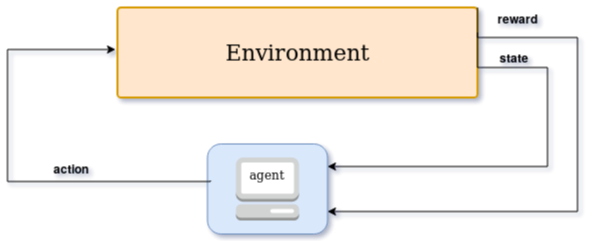
\includegraphics[width=90mm]{bilder/RLFramework.png}
\subsection{Elements of Reinforcement Learning}
\citet{Sut98} names 4 core elements of the reinforcement learning framework.

\textbf{Policy}

The behaviour of the agent within at any given time is determined by the \textit{policy}. A policy can roughly be described as a mapping of states to an action or a distribution over actions. 

\textbf{Reward Signal}

The problem posed by an environment is defined through the reward function. The goal of the learning agent is to receive the maximum accumulated future reward at any given time. One of the most important features of reinfocement learning is the fact, that rewards are often very delayed. Good opening moves in for example Chess will play a major role in winning the game, which however usually occurs at a much later stage. 

\textbf{Value Function}

The value of a state (or a state - action pair) describes how much more reward can be earned from this state onwards. Values represent the sum of the future rewards, and indicate the long term desirability of states.

\textbf{Environment Model}

In order to solve a problem, a model of the environment can be learned and used for planning. A model can be used to predict future states and rewards before they happen.
Model-based and model-free reinforcement learning methods, which explicitly learn by trial and error both play an important role in reinforcement learning.

\pagebreak

\subsection{Markov Decision Process} 

The sequential decision making process of the \textit{agent} can be more formally described as a Markov decision process (MDP).

The sequential decision making process is given by a sequence of states, actions and rewards:

$S_0, A_0, R_0, S_1, A_1, R_1, S_2, A_2, R_2, \dots, S_t,A_t,R_t, S_{t+1}$

Within this thesis a finite environment is assumed. We call a state \textit{Markov} or say it has \textit{Markov property} if it only depends on it's predecessor rather than the whole history.

$Pr(s_{t+1} = s', r_1 = r \mid s_t, a_t, r_t, s_{t-1},a_{t-1}, \dots ,r1,a0,s0) = Pr(s_{t+1} = s', r_1 = r \mid s_t,a_t)$

A finite discounted Markov decision process $MDP(S,A,P_a,R_a,\gamma)$ contains a finite set of states $S$, 
a finite set of Actions $A$,
the transition probablity to end up in state $s'$ if action $a$ is taken in state $s$ : 
$P^a_{s s'} = Pr(s_{t+1} = s' \mid s_t = s, a_t = a)$,
the reward function $R^a_{s s'}$,
and the discount factor $\gamma  \in [0,1)$, used to define the importance of immediate reward in contrast to future reward. 

\subsection{Deep Reinforcement Learning}
In contrast to simply mapping an input to an output value, deep learning algorithms contain so called \textit{hidden layers}.
For each layer the the weighted sum of units from the previous layer is computed as input. Usually a transformation or activation function is used on the input. Rectified linear units (ReLU), tanh or the sigmoid function can be named as popular activaton functions.
After feeding an input into the network and calculation an error value, the weights are ajusted through backpropagation.

Convolutional neural networks (CNN) were inspired by visual neuroscience and are great tools to process image data. CNNs usually contain convolutional layers, pooling layers and fully connected layers. Other relevant methods are recurrent neural networks (RNN) or long short term memory networks (LSTM).

Combining deep learning methods with reinforcement learning methods was a major breakthrough, enabeling reinforcement learning methods to be successfully applied to complex problems like those posed by the Atari 2600 console. \citep{deeprlLi}
\pagebreak